% Latex template: mahmoud.s.fahmy@students.kasralainy.edu.eg
% For more details: https://www.sharelatex.com/learn/Beamer

\documentclass{beamer}          % Document class

\usepackage{babel}        % Set language
\usepackage{verbatim}      % Set encoding

\mode<presentation>            % Set options
{
  \usetheme{default}          % Set theme
  \usecolortheme{default}         % Set colors
  \usefonttheme{default}          % Set font theme
  \setbeamertemplate{caption}[numbered]  % Set caption to be numbered
}

% Uncomment this to have the outline at the beginning of each section highlighted.
%\AtBeginSection[]
%{
%  \begin{frame}{Outline}
%  \tableofcontents[currentsection]
%  \end{frame}
%}

\usepackage{graphicx}          % For including figures
\usepackage{booktabs}          % For table rules
\usepackage{hyperref}          % For cross-referencing

\title{LRGrep}  % Presentation title
\subtitle{Engineering error messages for LR parsers}
\author{Frédéric Bour}                % Presentation author
\institute{Tarides, Inria}          % Author affiliation
\date{April 25, 2023}                  % Today's date

\begin{document}

% Title page
% This page includes the informations defined earlier including title, author/s, affiliation/s and the date
\begin{frame}
  \titlepage
\end{frame}

% Outline
% This page includes the outline (Table of content) of the presentation. All sections and subsections will appear in the outline by default.
\begin{frame}{Plan}
  \tableofcontents
\end{frame}

\AtBeginSection[]{
  \begin{frame}
  \vfill
  \centering
  \begin{beamercolorbox}[sep=8pt,center,shadow=true,rounded=true]{title}
    \usebeamerfont{title}\insertsectionhead\par%
  \end{beamercolorbox}
  \vfill
  \end{frame}
}

\section{Introduction}

\newcommand\pro{\item[$+$]}
\newcommand\con{\item[$-$]}

\begin{frame}{LR parsers}

  \begin{itemize}
    \pro \textbf{Declarative} \\
         {\small Work on a grammatical specification.}
    \pro \textbf{Efficient} \\
         {\small Analysis in $O(n)$.}
    \pro \textbf{Unambiguous} \\
         {\small Statically rule out ambiguities.}
    \pause
    \con \textbf{Limited expressiveness} \\
         {\small Some languages are not LR.}
    \con \textbf{Contrived grammars} \\
         {\small Some languages are hardly LR! (There might be a grammar...)}
    \con \textbf{Poor story for reporting errors} \\
         {\small Easy to locate a problem, hard to explain it.}
  \end{itemize}

\end{frame}

\begin{frame}[fragile]{Practical applications \& state of the art (1/2)}
  \begin{itemize}
    \item Bison \& Yacc (Johnson, 1975)
      \begin{itemize}
      \item Add rules for incorrect cases
      \item Non-local control flow (``{\em exceptions}''): the \textbf{error} {\em token}
    \end{itemize}
  \end{itemize}
\pause
\small
\begin{verbatim}
| LPAREN seq_expr error
    { unclosed "(" $loc($1) ")" $loc($3) }
\end{verbatim}
\pause
\begin{verbatim}
$ more foo.ml
(2 + )
$ ocamlc -c foo.ml
File "foo.ml", line 1, characters 5-6:
1 | (2 + )
         ^
Error: Syntax error: ')' expected
File "foo.ml", line 1, characters 0-1:
1 | (2 + )
    ^
This '(' might be unmatched
\end{verbatim}
\end{frame}

\begin{frame}[fragile]{Practical applications \& state of the art (2/2)}
  \begin{itemize}
    \item Merr (Jeffery 2003)
      \begin{itemize}
        \item Using sample inputs, associate error messages to {\em LR(1) states}
      \end{itemize}
    \pause
    \item Menhir (Pottier 2016)
      \begin{itemize}
        \item Enumerate examples to cover all error states
        \item Control reductions \only<3>{{\em ``(1 + 2''}}
        \item Successfully deployed in production (CompCert)
      \end{itemize}
    \pause
    \pause
    \item Menhir': {\em Faster reachability analysis for LR(1) parsers} (Bour \& Pottier, 2021)
      \begin{itemize}
        \item Speed-up enumeration by a factor 100x to 1000x
      \end{itemize}
  \end{itemize}
\end{frame}

\begin{frame}{Goal}

  Augment an LR grammar with a specification of error messages that is:
  \begin{itemize}
    \item declarative
      % Bison, Merr, Menhir, ...
      % Un langage spécifique auquel on peut donner plusieurs interprétations :
      % opérationnelle pour produire des messages d'erreur à l'exécution
      % statique, pour décider de la couverture, du code mort
    \item expressive (\& concise)
      % Contrairement à Merr et Menhir.
      % Factoriser des cas communs
      % Pour se référer à des éléments grammaticaux comme Bison
    \item easy to maintain
      % Contrairement à Merr et Menhir.
    \item separate from the grammar
      % Contrairement à Bison
  \end{itemize}
\end{frame}

\begin{frame}[t]{Core idea}

  \ \\ \

  Characterize error situations by matching the \textbf{LR stack} using \textbf{regular expressions}.

  \ \\

  \pause
  \begin{block}{Why the stack?}
    \begin{itemize}
      \item identify the current situation globally
      \item interpretable: it can be seen as the prefix of a {\em sentential form}.
    \end{itemize}
  \end{block}

  \only<3-4>{
  $$
  \begin{array}{rl}
    exp ::= & NUM \\
          | & \texttt{'(' } exp \texttt{ ')'} \\
          | & exp \texttt{ '+' } exp \\
  \end{array}
  $$
  }

  \only<4>{
  $$
  \begin{array}{rcl}
    ``(1 + 2) + 3 \cdot``  &\Rightarrow& exp  \texttt{ '+' } NUM\ \cdot
  \end{array}
  $$
  }

  \only<5->{
    \begin{block}{Why regular expressions?}
    \only<6>{
      \begin{itemize}
      \item the \textbf{stacks} themselves form a regular set
      \item the action of \textbf{reductions} form a regular set too
      \item lots of decidable properties: \textbf{exhaustivity}, \textbf{reachability}, \ldots
      \end{itemize}
    }
    \end{block}
  }
\end{frame}

\begin{frame}[t]{Regular expressions for LR stacks}

  \ \\ \

  $$
  \begin{array}{rlll}
    e ::=& X      & & \text{LR(1) states}\\
    | & e_1 e_2   & & \text{Concatenation}\\
    | & e_1 | e_2 & & \text{Disjunction}\\
    | & e^*       & & \text{Kleene star}\\
    | & [e\,]     & & \text{{\em Handles}}
  \end{array}
  $$

  \ \\ \

  \only<2-3>{
  \begin{itemize}
    \pause
    \item LR(1) states are denoted by LR items or incoming symbols
    \pause
    \item $[e\,]$ denotes the set of {\em handles} that reduce, in one or more steps, to a stack suffix matching $e$
  \end{itemize}
  }

  \only<4-6>{
  $$
  \begin{array}{rl}
    clause\ = & e\ \rightarrow action  \\
    \pause \pause \pause \pause
           | & e\ @\ \mathcal P(T\,) \rightarrow action \\
    \pause
    rule\ = & clause^*
  \end{array}
  $$
  }

\end{frame}

\section{Demonstration}

\begin{frame}{Application to OCaml grammar}
  Action!
\end{frame}

\begin{frame}{Integration with a Menhir parser}

  \begin{itemize}
    \item Files:
      \begin{itemize}
      \item Grammar, with extension \texttt{.mly}
      \item<2-> Error specification, with extension \texttt{.mlyl}
      \end{itemize}
    \item Compile-time:
      \begin{itemize}
        \item Menhir processes the \texttt{.mly} and produce a syntax analyser
        \item<2-> LRgrep processes the \texttt{.mlyl} and produce an error analyser
      \end{itemize}
    \item Run-time:
      \begin{itemize}
        \item The syntax analyser consume an input file
        \item Success case: it returns an AST (a semantic value)
        \item Failure case: it raises an exception \\
        \uncover<2->{
        \item The error analyser catches the exception and then
          inspects the state of the parser \\
            ($\approx$ like a debugger and a coredump)
        }
      \end{itemize}
  \end{itemize}

\end{frame}

\section{Theoretical foundation and concepts behind LRgrep}

\begin{frame}{Characterizing errors (1/3): langage complement}
  A grammar $G$ denotes a language $L$, a subset of the words on some alphabet $\Sigma$ (also known as terminals).
  $$
  [\![G\,]\!] = L \subset \Sigma^*
  $$

  \pause
  As a first approximation, an invalid input is any word that does not belong to the language:
  $$
  \Sigma^* / L
  $$

  \pause
  The grammar also gives structure to the words: the derivations.
  \\
  Can we give some structure to the errors?
\end{frame}

\begin{frame}{Characterizing errors (2/3): the error front}
  An LR parser consumes the input from left to right, and fail as early as possible (as soon as the input is not a prefix of any word of the language, {\em the viable-prefix property}).

  % Attention aux conflits cependant !
  % C'est grâce à ça qu'on peut raporter au moins la position de l'erreur.

  \pause
  Lets consider this set of minimal failing prefixes:

  $$
  \mathcal E_L = \left\{ (u, t) \in \Sigma^*\times\Sigma\ \big|\
    \text{viable}(u) \wedge \neg \text{viable}(u.t)
  \right\}
  $$
  \qquad where $\text{viable}(u) = \exists v \in \Sigma^*,\ u.v \in L$
  \pause
  \\ \ \\
  In this set of pairs $(u,t)$, $u$ is a valid prefix and $t$ is a terminal that will cause the analysis to fail.
\end{frame}

\begin{frame}[t]{Characterizing errors (3/3): regularisation}

  \ \\

  Since the $u$ are valid prefixes, we can feed them to a parser and get a {\em stack}. We call this operation $im$ and define:

  $$
  \mathcal E_G = \left\{\ (im(u), t)\ \mid\ (u, t) \in \mathcal E_L\ \right\}
  $$

  \pause
  \begin{block}{Theorem (Aho \& Ullman, 1972)}
    The set of all \only<-2>{\em viable prefixes of the right sentential forms of a grammar}\only<3->{\textbf{stacks of an LR automaton}} is a regular language.
  \end{block}

  \pause
  \pause

  \ \\
  Therefore $\mathcal E_G$ is a regular set!

  \textbf{Good news:} many properties are decidable on regular sets, we have
  many tools to work with them (such as regular expressions).
\end{frame}

\begin{frame}{Intuition on ``Shift-Reduce'' parsers}

  {\em Bottom-up} analysis using a stack:

  \begin{itemize}
    \item the input is consumed left to right ({\em push})
    \item the derivation is built starting from the leaves,
          that are progressively rooted ({\em pop} leaves, {\em push} node)
    \item the stack saves the intermediate derivations
    \item the analysis ends with the root of the derivation on the stack
  \end{itemize}

  \pause

  Example with a minimalist grammar:
  $$
  \begin{array}{rl}
    exp ::= & num \\
          | & exp\,+ exp \text{, right associative}\\
  \end{array}
  $$

  Let's analyse the expresssion $1+2+3$.
\end{frame}

\begin{frame}[t]{Intuition on ``Shift-Reduce'' parsers}
  \begin{columns}[T]
    \begin{column}{.5\textwidth}
    \scalebox{0.8}{
      \begin{tabular}{|l|l|}
        \hline
        Stack & Input \\
        \hline
        $\emptyset$ & \texttt{num + num + num \$} \\
        \uncover<3->{\texttt{\only<4>{\underline}{num}}
                                              & \texttt{+ num + num \$}} \\
        \uncover<5->{\texttt{exp}             & \texttt{+ num + num \$}} \\
        \uncover<6->{\texttt{exp +}           & \texttt{num + num \$}} \\
        \uncover<7->{\texttt{exp + \only<8>{\underline}{num}}
                                              & \texttt{+ num \$}} \\
        \uncover<9->{\texttt{exp + exp}       & \texttt{+ num \$}} \\
        \uncover<10->{\texttt{exp + exp +}    & \texttt{num \$}} \\
        \uncover<11->{\texttt{exp + exp + \only<12>{\underline}{num}} & \texttt{\$}} \\
        \uncover<13->{\texttt{exp + \only<14>{\underline}{exp + exp}} & \texttt{\$}} \\
        \uncover<15->{\texttt{\only<16>{\underline}{exp + exp}}       & \texttt{\$}} \\
        \uncover<17->{\texttt{exp}             & \texttt{\$}} \\
        \uncover<18->{\texttt{exp \$}          & $\emptyset$} \\
        \uncover<19->{\texttt{goal}            & $\emptyset$} \\
        \hline
      \end{tabular}
    }
    \end{column}

    \begin{column}{.5\textwidth}
    \vspace{-10pt}
    \only<1-2>{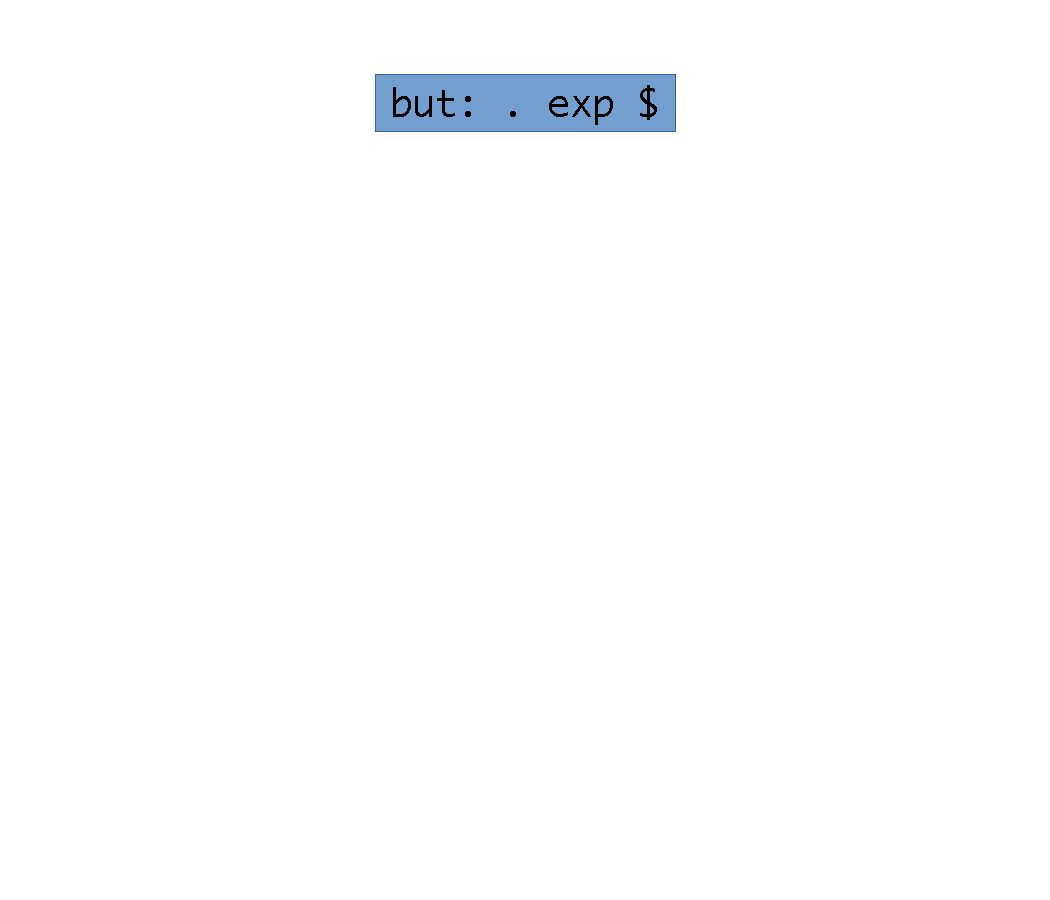
\includegraphics[page=1,width=160pt]{dfa.en.pdf}}
    \only<3>{\includegraphics[page=2,width=160pt]{dfa.en.pdf}}
    \only<4>{\includegraphics[page=3,width=160pt]{dfa.en.pdf}}
    \only<5>{\includegraphics[page=4,width=160pt]{dfa.en.pdf}}
    \only<6>{\includegraphics[page=5,width=160pt]{dfa.en.pdf}}
    \only<7>{\includegraphics[page=6,width=160pt]{dfa.en.pdf}}
    \only<8>{\includegraphics[page=7,width=160pt]{dfa.en.pdf}}
    \only<9>{\includegraphics[page=8,width=160pt]{dfa.en.pdf}}
    \only<10>{\includegraphics[page=9,width=160pt]{dfa.en.pdf}}
    \only<11>{\includegraphics[page=10,width=160pt]{dfa.en.pdf}}
    \only<12>{\includegraphics[page=9,width=160pt]{dfa.en.pdf}}
    \only<13>{\includegraphics[page=11,width=160pt]{dfa.en.pdf}}
    \only<14>{\includegraphics[page=9,width=160pt]{dfa.en.pdf}}
    \only<15>{\includegraphics[page=11,width=160pt]{dfa.en.pdf}}
    \only<16>{\includegraphics[page=13,width=160pt]{dfa.en.pdf}}
    \only<17>{\includegraphics[page=14,width=160pt]{dfa.en.pdf}}
    \only<18>{\includegraphics[page=15,width=160pt]{dfa.en.pdf}}
    \only<19>{\includegraphics[page=16,width=160pt]{dfa.en.pdf}}
    %
    %\only<1,2,8,12,14,16>{\uncover<0>{X}}%
    \only<3>{Shift \texttt{num}}%
    \only<4-5>{Reduce \texttt{exp: num}}%
    \only<6>{Shift \texttt{+}}%
    \only<7>{Shift \texttt{num}}%
    \only<8-9>{Reduce \texttt{exp: num}}%
    \only<10>{Shift \texttt{+}}%
    \only<11>{Shift \texttt{num}}%
    \only<12-13>{Reduce \texttt{exp: num}}%
    \only<14-15>{Reduce \texttt{exp: exp + exp}}%
    \only<16-17>{Reduce \texttt{exp: exp + exp}}%
    \only<18>{Shift \texttt{\$}}%
    \only<19>{Reduce \texttt{goal: exp \$}}%

    \texttt{\\
    \only<1-2>{goal: . exp \$}
    \only<2>{
      \rule{\textwidth}{0.5pt}
      exp: . num \\
      exp: . exp + exp
    }
    \only<3,7,11>{%
      exp: num .
    }
    \only<5>{%
      goal: exp . \$ \\
      exp: exp . + exp
    }
    \only<6,10>{%
      exp: exp + . exp
      \rule{\textwidth}{0.5pt}
      exp: . num \\
      exp: . exp + exp
    }
    \only<9,13-16>{%
      exp: exp + exp . \\
      exp: exp . + exp
    }
    \only<17>{goal: exp . \$}
    \only<18>{goal: exp \$ .}
    \only<19>{Accept (goal .)}
    }
    \end{column}
  \end{columns}
\end{frame}

\begin{frame}[t]{Regular expressions for LR stacks}

  $$
  \begin{array}{rlll}
    e ::=& X      & & \text{LR(1) states}\\
    | & e_1 e_2 & & \text{Concatenation}\\
    | & e_1 | e_2 & & \text{Disjunction}\\
    | & e^*       & & \text{Kleene star}\\
    \only<1-2>{| & \ldots &&}
    \only<3->{| & [e\,]       & & \text{{\em Handles}}}
  \end{array}
  $$

  \pause
  \begin{minipage}{10cm}
    \vspace{1cm}
  \only<1-2>{
    \uncover<2>{
    Enough to identify specific stacks, too fine-grained in practice:
    no way to talk about reductions.
    }
  }
  \end{minipage}
  \begin{minipage}{10cm}
    \vspace{1cm}
  \only<3->{
    \uncover<4->{
      The new construct $[e\,]$ to denote a set of {\em handles}
      that can reduce, in one or more steps, to a stack suffix matching $e$.
    }

    \

    \uncover<5->{
    In our example:
    $[exp\,] = num\,\big|\,exp + [exp\,]$
    }
  }
  \end{minipage}
\end{frame}

\begin{frame}{Also...}
  The implementation also have extra features useful in practice:
  \begin{itemize}
    \item captures (refer to semantic values and locations on the stack)
    \item ``greedy'' repetitions of Kleene-star and handles (should we keep the longest or the shortest result?)
    \item filters to restrict states to specific {\em items}
    \item constraints on lookahead tokens (the $t$'s of the $\mathcal E_G$ set)
    \item partial rules (like ``guarded'' patterns)
    \item total order on clauses to resolve ambiguities
    \item \ldots
  \end{itemize}

\end{frame}

\section{Practical work}

\begin{frame}{Adding an error message to OCaml}

  To add a new error message:
  \begin{itemize}
    \item start from an example, usually an issue reported by a user
    \item throw this example to an ``interpreter'' that provides information on the LR stack and on {\em handles}
    \item then its our work to generalise from this example
  \end{itemize}
  \pause
  \begin{block}{If you happen to use OCaml: help!}
    Don't hesitate to report the ``interesting'' errors you encounter.
  \end{block}
\end{frame}

\section{Conclusion}

\begin{frame}{Conclusion}
  LRgrep is a new DSL ({\em domain specific language}) to identify error of LR parsers.

\

  The early results are encouraging: we can precisely identify a rather large class of errors for the OCaml grammar. Tools are provided to help the author work out error patterns.

\

  The approach builds upon a new application for a well-understood theory, which gives hope for rapid progress.

\end{frame}

\begin{frame}{Future work}

  The main feature that is missing is a tool to test coverage of a grammar:
  which grammatical constructs have no associated errors, which rules are unreachable.

  We identified two difficulties:
\begin{itemize}
  \item computing the coverage itself
  \item displaying the outcome to the user
\end{itemize}

This feature will be crucial to maintain the specifications (as a grammar evolve).

\

\pause
Application to other grammars. We started looking at other candidates (only Menhir grammars for now): Catala, EasyCrypt, ...
An external contributor is looking at Lua grammar.

\end{frame}

\begin{frame}{That's all, thanks!}

  Thanks for your attention.

\end{frame}

\end{document}
